%!TEX root = ./lec04_access_methods.tex

%
% ---------------------------------------------------------------------------
%
\begin{frame}{Heap Files: Implementation and Access Cost}

Heap files are similar to singly-linked lists, which are easy to maintain. 

\vskip2em 

\begin{center}
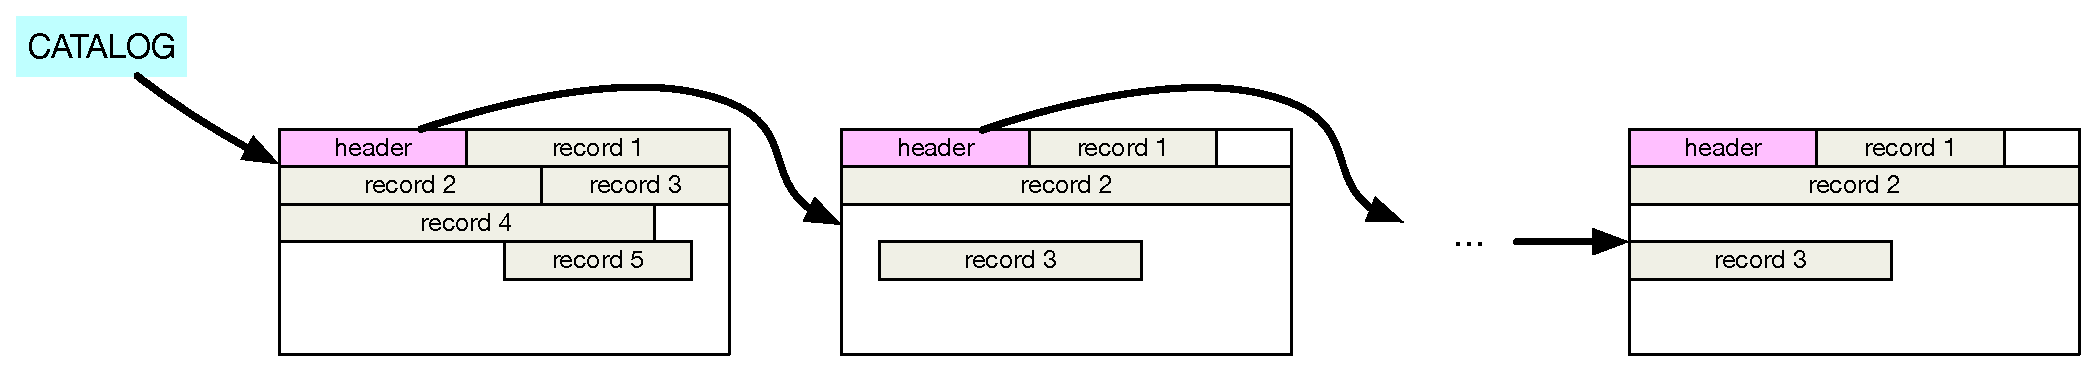
\includegraphics[width=\textwidth]{figures/heap_file_with_catalog.eps}
\end{center}

\vskip1em

All the DBMS needs to record (in the Catalog) is a pointer to the first block in the file.

Each block has its own header for metadata, including, among other things, links to the next block in the chain.

\end{frame}


\begin{frame}{Access costs}

Recall from CMPUT204 that we measure computational costs by in terms of functions that bound \textbf{how many operations} the algorithm requires to complete.

For algorithms dealing with data structures in memory, we typically count accesses to memory.

\vskip1em

\begin{block}{\alert{Computational Cost units}}
Because I/O is so slow, we measure the \textit{cost} as a function of \textbf{how many disk blocks need to be read or written} to perform the operation.
\end{block}
\end{frame}


\begin{frame}

Which kinds of access are supported?

\textbf{Inserting} a new record.

\textbf{Searching} for a record, given a search key.
\begin{itemize}[-,topsep=-0.5em]
\item Example: find movies with \lstinline[style=cmput391]{director='Ivan Reitman'}
\end{itemize}

\textbf{Deleting} or \textbf{updating} a record.

\vskip1em

Note that before we can update or delete a record, we need to first \emph{find} it. The costs for these operations in the following slides will include the search cost. 
\end{frame}


\begin{frame}

\begin{center}
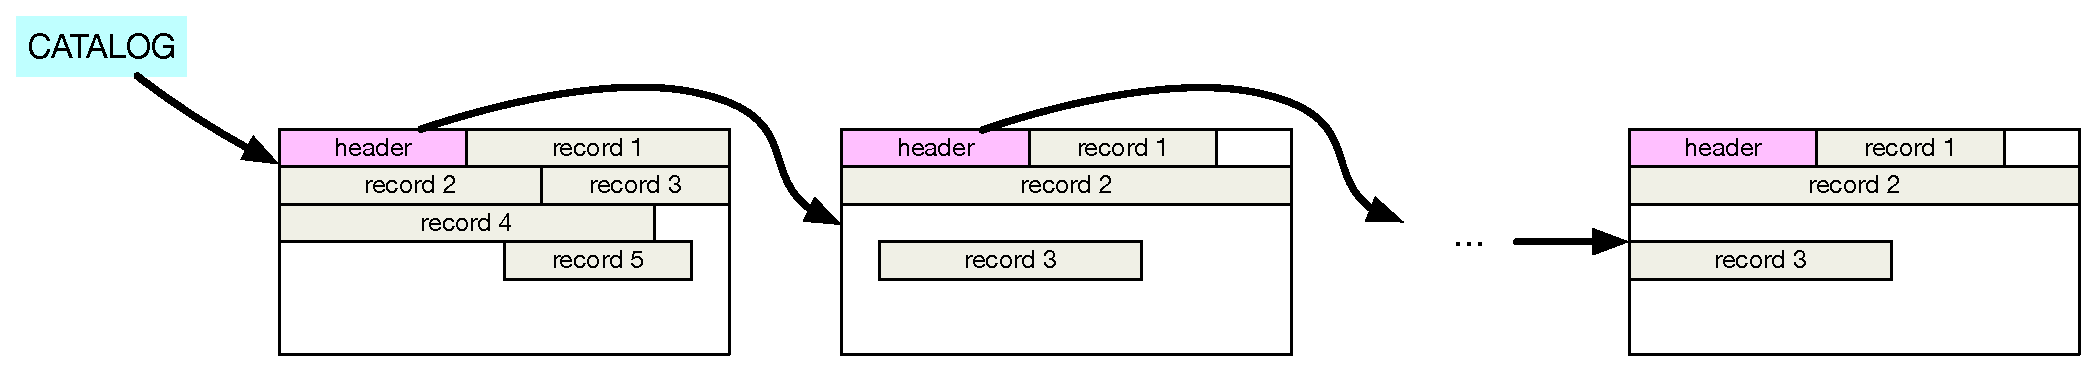
\includegraphics[width=\textwidth]{figures/heap_file_with_catalog.eps}
\end{center}

\textbf{Inserting a new record in a Heap File:}
\begin{itemize}[-,noitemsep,topsep=-0.5em]
\item If there is room in the first block, add the record there.
\item Otherwise, allocate another block to the file, add the record there, and link the new block to the previous first block.
\end{itemize}

\vskip2em

\begin{center}
\fbox{The \textbf{cost} of inserting a new record is $O(1)$}
\end{center}
\end{frame}

%
% ---------------------------------------------------------------------------
%
\begin{frame}

\begin{center}
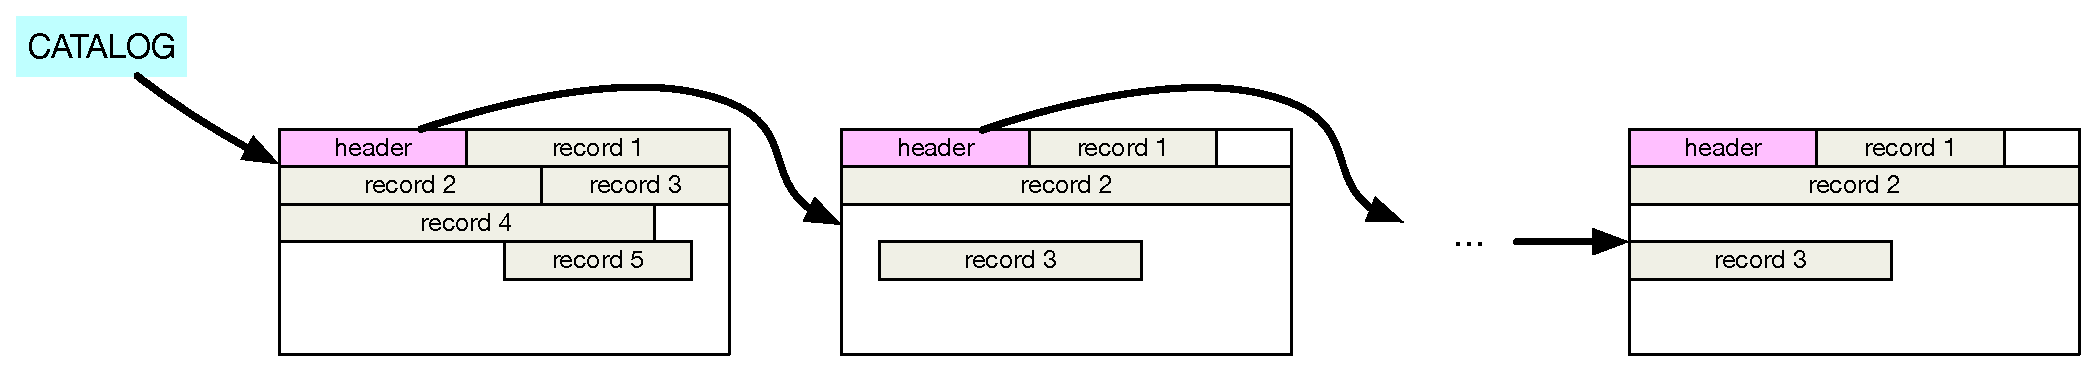
\includegraphics[width=\textwidth]{figures/heap_file_with_catalog.eps}
\end{center}

\vskip1em

\textbf{Searching for a record in a Heap File} with $N$ in blocks.
\begin{itemize}[-,noitemsep,topsep=-0.5em]
\item Traverse all blocks, starting from the first block, following pointers until the record is found (or we exhaust the last block)
\end{itemize}
 
\vskip2em

\begin{center}
\fbox{The \textbf{cost} of finding a record is $O(N)$.}
\end{center}

\end{frame}

\begin{frame}

\begin{center}
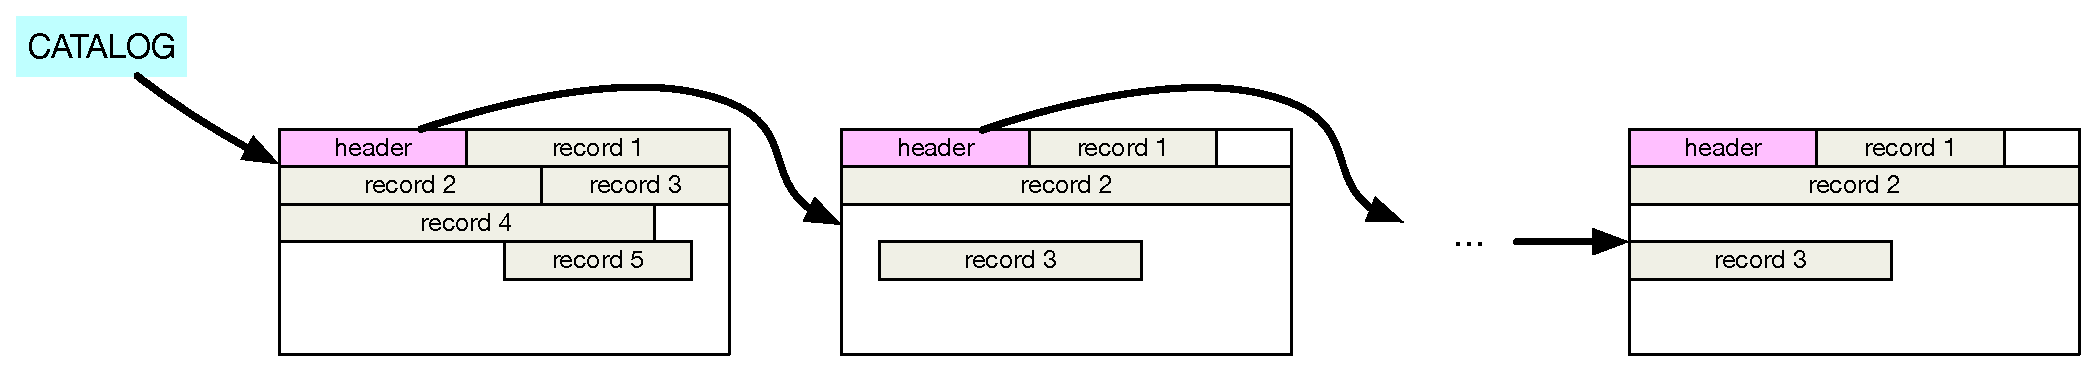
\includegraphics[width=\textwidth]{figures/heap_file_with_catalog.eps}
\end{center}

\vskip1em

\textbf{Deleting or updating a record in a Heap File} with $N$ blocks:
\begin{itemize}[-,noitemsep,topsep=-0.5em]
\item Find the record first (cost $O(N)$), and modify it, or remove it from the block.
\item For deletions: if the block becomes empty, link the previous block to the next in the chain (unless the deletion happens in \emph{last} block).
\end{itemize}

\vskip2em

\begin{center}
\fbox{The \textbf{cost} of deleting a record is $O(N)~$\footnote{Again, because of the search step.}.}
\end{center}
\end{frame}

%
% ------------------------------------------------------------------------------------------------------------------------------
%

\begin{frame}{Sequential Files}


\textbf{Sequential file} are chains of blocks in which the records are \emph{sorted} on a predefined set of attributes, both \emph{within} and \emph{across} blocks.

Tables with primary keys are always stored using sequential files with the primary key as the sorting attributes.

\vskip1em

\begin{columns}[onlytextwidth]
\begin{column}{0.4\textwidth}

Example: sequential file for table \lstinline[style=cmput391]{Movie} sorted by primary key (\lstinline[style=cmput391]{title, year}).

\vskip4em
~

\end{column}
\begin{column}{0.525\textwidth}
\begin{tikzpicture}
\node [anchor=north west] at (0,0) {\scalebox{0.9}{\usebox\SequentialFileMovieTitleYear}};
\end{tikzpicture}
\end{column}
\end{columns}
\end{frame}

%
% ---------------------------------------------------------------------------
%
\begin{frame}{Access cost of Sequential Files}

Searches and deletions are the same as for heap files.

\vskip2em

For \textbf{insertions} on a file with $N$ blocks, we now need to:
\begin{enumerate}[(1),noitemsep,topsep=-0.5em]
\item Find the block where to insert the new record (at cost $O(N)$).
\item Insert the record if there is room, otherwise \alert{rearrange the file}.
\end{enumerate}

\vskip1em

Two ways of rearranging the file:
\begin{itemize}[-,topsep=-0.5em,noitemsep]
\item moving existing records
\item creating a new empty block
\end{itemize}

\end{frame}

%
% ---------------------------------------------------------------------------
%

\begin{frame}{Insertion by rearranging records}

Example: inserting \qquad \raisebox{0.75em}{\scalebox{0.9}{\usebox{\MovieVI}}}

\vskip1em

\begin{columns}[onlytextwidth]
\begin{column}{0.475\textwidth}

\centering \large Before \\[1em]

\begin{tikzpicture}
\node [anchor=south west] at (0,0) {\scalebox{0.8}{\usebox\SequentialFileMovieTitleYear}};
\coordinate (Empty) at (0.2,0.25); 
\coordinate (Wadja) at (0.2,0.5);
\coordinate (LiT) at (0.2,1.25); 
 \path[red, ->,>=stealth'] 
    (Wadja.south) edge[bend right=35] (Empty)
    (LiT) edge[bend right=35] (Wadja.north);
\end{tikzpicture}
\end{column}
\begin{column}{0.475\textwidth}

\centering \large After \\[1em]

\begin{tikzpicture}
\node [anchor=north west] at (0,0) {\scalebox{0.8}{\usebox\SequentialFileMovieTitlYearUpdated}};
\end{tikzpicture}
\end{column}
\end{columns}

\vskip1em

In the worst case scenario, need to keep moving records all the way to the end of the file.

\begin{center}
\fbox{\parbox{0.8\textwidth}{\textbf{cost}: $O(N)$ to rearrange the records in the file; \\~~~~~$O(N)$ to find the block where to make the insertion.}}
\end{center}

\end{frame}


%
% ---------------------------------------------------------------------------
%

\begin{frame}{Insertion by creating a new block}

Example: inserting \qquad \raisebox{0.75em}{\scalebox{0.9}{\usebox{\MovieVI}}}

\vskip2em

\begin{columns}[onlytextwidth]
\begin{column}{0.475\textwidth}

\centering \large Before \\[1em]

\begin{tikzpicture}
\node [anchor=south west] at (0,0) {\scalebox{0.8}{\usebox\SequentialFileMovieTitleYear}};
\end{tikzpicture}
\end{column}
\begin{column}{0.475\textwidth}

\centering \large After \\[1em]

\begin{tikzpicture}
\node [anchor=north west] at (0,0) {\scalebox{0.8}{\usebox\SequentialFileMovieTitlYearUpdatedTWO}};
\end{tikzpicture}
\end{column}
\end{columns}

\vskip1em

\begin{center}
\fbox{\parbox{0.8\textwidth}{\textbf{cost}: $O(1)$ to modify the file; \\~~~~~$O(N)$ to find the block where to make the insertion.}}
\end{center}
\end{frame}

%
% ---------------------------------------------------------------------------
%

\begin{frame}
What about \textbf{updates} to a record in a sequential file?

\vskip1em

\textbf{Case \#1}: The update does not change the sort attributes in the record.
\begin{itemize}[-,topsep=-0.5em]
\item In this case the record remains in the same block as it was\footnote{Unless, of course, the file uses variable length records and the update makes the record too large to fit in the block! In which case a new block must be added to the file.}
\end{itemize} 

\vskip1em

\textbf{Case \#2}: The update does change the sort attributes in the record.
\begin{itemize}[-,topsep=-0.5em]
\item This case is best handled by a deletion of the ``old'' record (before the update) followed by the insertion of the ``new'' record (after the update).
\end{itemize} 

\end{frame}

%
% ---------------------------------------------------------------------------
%

\begin{frame}{Heap vs Sequential Files}
\label{costs_heap_sequential_files}

Both are based on singly-linked lists.

\vskip0.5em

Heap files are better for insertions, but all other operations cost the same in both. If $N$ is the size (in blocks) of the file, then:

\begin{center}
% \large
\begin{tabular}{l | c | c}
& Heap & Sequential\\
\hline\hline
insertion & $O(1)$ & $O(N)$\\
\hline
search & $O(N)$ & $O(N)$\\
\hline
deletion & $O(N)$ & $O(N)$\\
\hline
update & $O(N)$ & $O(N)$
\end{tabular}
\end{center}

\vskip1em

\begin{block}{We need indexes!}
Indexes are needed to cut down the $O(N)$ time to find tuples inside the table file (heap or sequential).
\end{block}

\end{frame}

\begin{frame}

Sequential files can have many quasi-empty blocks after many insertions... which wastes space and (more importantly) I/O operations. 

\vskip1em

\begin{columns}[onlytextwidth]
\begin{column}{0.3\textwidth}
Before:
\end{column}
\begin{column}{0.7\textwidth}
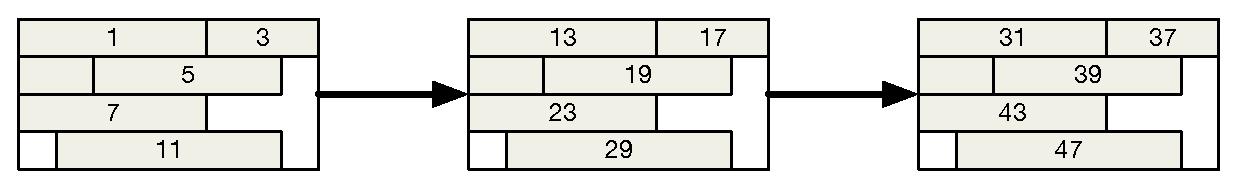
\includegraphics[width=1\textwidth]{figures/seq_file_update_ex1.eps}
\end{column}
\end{columns}

\vskip3em

\pause

\begin{columns}[onlytextwidth]
\begin{column}{0.3\textwidth}
After:
\end{column}
\begin{column}{0.7\textwidth}
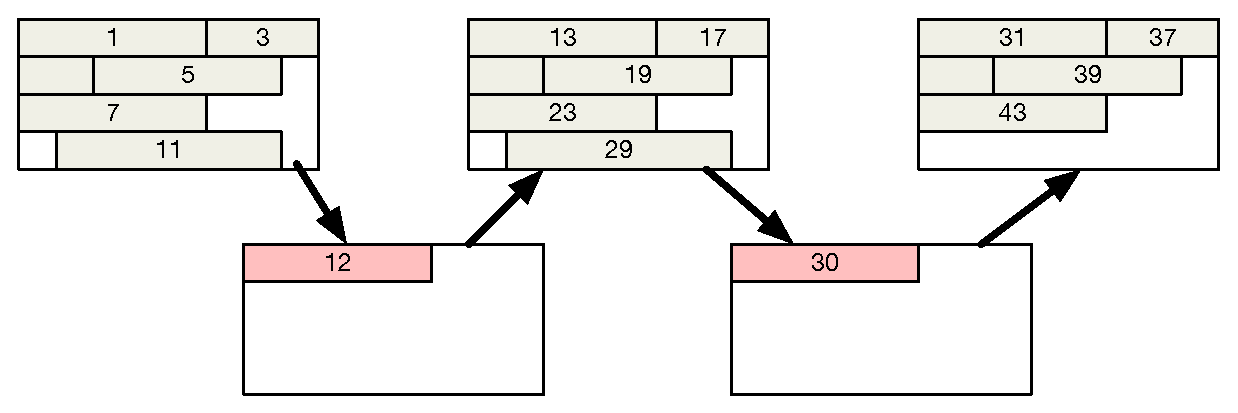
\includegraphics[width=1\textwidth]{figures/seq_file_update_ex2.eps}
\end{column}
\end{columns}

\vskip1em

This can be fixed by \textbf{periodically} taking the database \emph{offline} and re-building the file.

\end{frame}
